\documentclass[11pt]{article}
\usepackage{graphicx}
\usepackage{geometry}                		% See geometry.pdf to learn the layout options. There are lots.
                 		% ... or a4paper or a5paper or ... 
%\geometry{landscape}                		% Activate for rotated page geometry
%\usepackage[parfill]{parskip}    		% Activate to begin paragraphs with an empty line rather than an indent
			% Use pdf, png, jpg, or eps§ with pdflatex; use eps in DVI mode
								% TeX will automatically convert eps --> pdf in pdflatex		
\usepackage{amssymb}
\usepackage{float}
\usepackage{caption}
\usepackage{subcaption}
\usepackage{amsmath}
\usepackage{amssymb}


\begin{document}


\begin{center}
{\bf{\huge{Motion Control Manual for pSCT Telescope}}}

\vspace{0.1in}
Last updated July, 2016

\vspace{0.3in}
{\it{\underline{Abstract:}}} We detail the operation and troubleshooting methods for the telescope motion control system.

\end{center}

\tableofcontents

\vspace{0.2in}


\section{Overview}

This manual details the system in place to control the mechanical motion of the telescope inner structure.
The motion is controlled by three stepper motors as shown in Fig. \ref{fd2}, and allows up to 5 inches of motion along each independent stepper axis. 
A web interface hosted on an Arduino Yun interfaces and commands these steppers.


\section{Important Warnings/Notes}

First, some important warnings:
\begin{enumerate}
	\item Once the motion control set screws have been locked (this is done after the camera is aligned) {\bf DO NOT MOVE} the camera in any way except all forward or all backward (called vertical or along axis in the UI).
	Moving in any other way will break or bend things!
	\item Every time that you begin moving the camera, start small.  Test each motor individually +/-100 steps.  
		If you don't see a motor move, you can test that there isn't a problem with the screw by using a 1/2 inch socket to move the alignment screw for that motor.
		Use the socket on the front side of the screw (opposite the motor).
	\item If you need to turn off motion very quickly in the case of an emergency (someones fingers in the way of motion, etc) you can click the green button on the electronics box.
		 This will kill the power to the arduino and the motors and everything will stop immediately.
		 Simply click the button back on and everything should power up without problems.
\end{enumerate}


\section{Startup Procedure}

\begin{itemize}
	\item Power the electronics box.  You'll need to make sure that the green button on the side of the box is clicked-in.
	\item Navigate to the ip address that hosts the control html: [IP]/sd/MotionControl/
	\item You are now able to move the camera along its axis (i.e. all motors together).  
		If you instead need to align it, click the 'ALIGNMENT MODE' button and follow the instructions in Sec. \ref{alignSec}.
	\item Note that your first movement command will not go through.  
		You will be asked by the arduino to authenticate (default is root, arduino).
	\item Select the direction (+/-) and number of steps to move and have at it.  
		You will see a message that the movement completed successfully if there are no problems.
\end{itemize}


\section{User Interface Commands}
\begin{enumerate}
	\item[GETRNG:] Load the camera range into the UI engine from the file on the Yun sd card. (range.txt)
	\item[GETPOS:] Load the camera position into the UI engine from the file on the Yun sd card. (position.txt)
	\item[GETALGN:] View the camera alignment position stored on the Yun sd card.
	\item[SETALGN:] Write the current position as the alignment position to the Yun sd card. (alignment.txt)
	\item[Vertical:] Move all three motors.
	\item[Pitch:] Move motor A in the requested direction. Move motor B in the opposite direction.
	\item[Roll:] Move both motors A and B in the same direction.
	\item[A only:] Move only motor A.
	\item[B only:] Move only motor B.
	\item[C only:] Move only motor C.
	
	\item[Setting Range:] If for some reason the range hasn't been set correctly, do the folowing:
	\begin{enumerate} 
		\item[1.]SSH into the Yun.
		\item[2.]Use vi to manually change the position.txt file (in /mnt/sda1/) to "20000L20000L20000".
		\item[3.]Use vi to manually change the range.txt file (in /mnt/sda1/) to "20000L20000L20000".
		\item[4.]Hit GETPOS on the webpage.
		\item[5.]Use the webpage to move the camera all the way back to the -Z limit.
		\item[6.]Change the position.txt file to "0L0L0".
		\item[7.]Hit GETPOS on the webpage.
		\item[8.]Use the webpage to move the camera all the way to the +Z limit.
		\item[9.]Hit GETPOS on the webpage.
		\item[10.]Manually change the range.txt file to the current position.
	\end{enumerate}
\end{enumerate}

\begin{figure}[h]
\begin{center}
\includegraphics[width = 4.5in]{camerapic.png}
\caption{}  
\label{fd2}
\end{center}
\end{figure}


\section{Alignment Procedure}
\label{alignSec}
\begin{enumerate}
	\item Navigate to the MotionControl webpage from the (arduino ip)/sd webpage.
	\item Navigate to the alignment mode webpage (password is cta).
	\item Use the webpage to move the camera to a position where it is aligned.
	\item Hit SETALGN to save the alignment position.
\end{enumerate}

\section{Troubleshooting}
If power is lost at any time, it might be the case that one of the following files gets deleted: position.txt, range.txt, alignment.txt\\[15pt]
Each of these files sits inside the directory /mnt/sda1\\[15pt]
If position.txt, or range.txt is missing:
\begin{enumerate}
\item[1.] Go into alignment mode if not there already and find the camera range (see "Setting Range" above).
\item[2.] Hit GETALGN to request the stored alignment position.
\item[3.] Manually move the camera to the alignment position.
\item[4.] Go back to the normal operation mode.
\end{enumerate}
If alignment.txt is missing realign the camera. Sorry :/. (This should never happen)

\section{Replacing a Yun}
\begin{enumerate}
\item Plug Yun into laptop via micro usb.
\item Look for the Yun's wifi network. If it doesn't appear, hold the wlan reset button until it blinks.
\item If the Yun's wifi network still doesn't appear try plugging the Yun ethernet into your LAN and connect to the Yun or Linino's network. Continue below as appropriate.\\
\item Are you using a Linino or Arduino?
        	\begin{itemize} 
		\item {\textbf{Linino:}} Open a browser and go to 192.168.240.1 and login to the Linino web UI. The default password is 'doghunter'.
		\item {\textbf{Arduino:}} Open a browser and go to arduino.local and login to the Arduino web UI. The default password is 'arduino' or 'arduino1'.
	\end{itemize}
\item \textbf{Continue Here:} Click on the advanced configuration at the top of the page.
\item Go to the network tab and click edit on the WAN panel.
\item Switch the network protocol to static ip.
\item Enter LAN ip reserved for the Yun along with the gateway ip and network mask. Hit save.
\item If required go to the wifi panel and disable the wifi.

\item If desired, set up the LAN to forward incoming requests from some port to the Yun ip.\\
\item \textbf{Loading the sketch:} If the previous Yun's sd card is still accessible just put it into the new Yun. Otherwise get a fresh sd card and download the Yun sd expander sketch (Google it).
\item If necessary find the Yun's ip address on the LAN and go that ip in your web browser. Then open up the Arduino IDE and select that same ip as the port. Upload the sd expander (and or the motion control sketch) if necessary.

\item After loading from the Arduino IDE you should see all the green lights on for the three motor drivers (not flashing).  
The motor drivers are located in the electronics box, see the wiring diagram below.

\item {\textbf{If you are using a Linino:}}  If the Ardiuno is a Linino you may have to create a symbolic link for the OS to know where to look for the website.  
After these steps you should be able to load the webpage via [ArduinoIP] / [sd].  
If you can already connect, all is good already.
	\begin{itemize}
		\item ssh -Y root@[IP address]
		\item cd /www/
		\item ln -s /mnt/sda1/sd
	\end{itemize}
\end{enumerate}


\section{Removing the Inner Camera Structure}
We show here a step-by-step of removing the inner camera structure.  
Note that a lifting crane is absolutely necessary, the inner structure is very heavy.

\begin{enumerate}
\item Ratchet down bottom screws (screws pushing up on the holding pins)
\item Move camera all the way forward
\item Allen wrench off the top piece holding in the pin.  See Figure \ref{fd1}.
\item Jiggle to get the ball to disconnect
\item Pop top ball joint out.  Now the top tilts forward.  See Figure \ref{fd2}.
\item Pull it up straight.
\item Pop out one of the two bottom pins (take it out 'leg-by-leg'). 
\item Lift manually out the other side pin
\item Don't drop it.  
\end{enumerate}

\section{Mounting the Inner Camera Structure}
We show here a step-by-step to mount the inner camera structure.  
Note that a lifting crane is absolutely necessary, the inner structure is very heavy.

\begin{enumerate}
\item Move bottom motors all the way forward, the top motor all the way back.
\item Make sure the screws for the holding pins are ratcheted down.
\item Put one lower ball joint in place
\item Bring the whole inner structure down to sink that one in
\item Pivot to put the other lower pin in
\item Now lower the inner structure all the way down until it is resting (you need clearance for the top pin)
\item Put the top ball pin in all the way and hold it there (you may have to ratched the screw up all the way)
\item Pivot the camera structure to put the ball into place 
\item Attach the ball pin holding frame with 1/8 inch allen
\item Ratchet up the bottom two nuts
\end{enumerate}


\begin{figure}[h]
\begin{center}
\includegraphics[width = 3in]{photo_2.png}
\end{center}
\caption{}  
\label{fd1}
\end{figure}


\begin{figure}[h]
\begin{center}
\includegraphics[width = 3in]{photo_3.png}
\end{center}
\caption{}  
\label{fd2}
\end{figure}

\begin{figure}[h]
\begin{center}
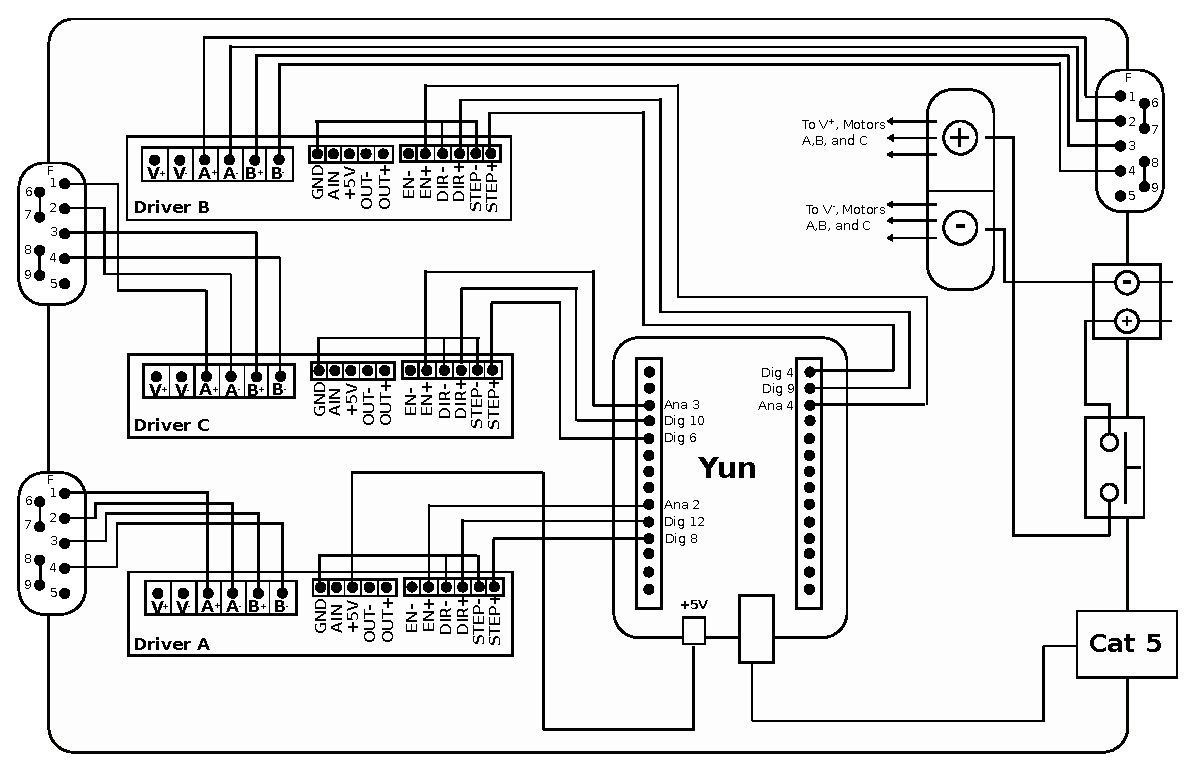
\includegraphics[width = 5.5in]{wiringDrawing.eps}
\caption{Wiring diagram for the electrical control box.}  
\label{fd2}
\end{center}
\end{figure}


\section{Fan Assembly Details}

The camera cooling system consists of two banks of 4 fans blowing through a water cooled radiator.
Each fan is an ebm-pabst model DV 6224 and the power is supplied by an Acopian power supply.
The fan banks run at a nominal voltage of 24V and draws 7A.
Figure \ref{fanPic} shows the terminal to connect the fan bank wires properly.


\begin{figure}[h]
\begin{center}
\includegraphics[width = 4in]{fanWiring.jpg}
\caption{Terminal block for fan assembly wiring.}  
\label{fanPic}
\end{center}
\end{figure}

\newpage
\section{Tools in the Telescope Kit}

All the tools needed to drive each screw or bolt on the camera should be included in the camera toolbox. 
Additionally, there are spares for all the major components and connectors.
Have a look there first if you need something.
Here is what should be in there:

\begin{itemize}
	\item 3/4 inch flexible ratchet wrench with tape -- ball joint vertical centering screws for alignment
	\item 9/16 inch flexible ratchet wrench with tape -- ball joint horizontal centering screws for alignment
	\item 5/16 inch allen -- bolts for ball joint mount
	\item 7/32 inch allen -- Screw assembly bolts
	\item 2.5 mm allen -- slides
	\item 7/16 inch wrench (2x) -- screw flange bolts to connect screw to frame
	\item 3/16 inch wrench (2x) -- small wrenches for electronics box nuts
	\item 1/16 inch allen -- set screws for motor pins
	\item Phillips or flathead screwdriver -- everything else
	\item Spare $\mu$SD card
	\item Spare stepper motor driver + wiring terminals
	\item Spare stepper motor
	\item Touch-up paint and grease
	\item Spare electronics box pars (switch, ethernet mount, etc.)
\end{itemize}

\end{document}
